\documentclass[12pt,twoside, a4paper, twocolumn]{article}
\usepackage[utf8]{inputenc}
\usepackage[brazil]{babel}
\usepackage[margin = 0.5in]{geometry}
\usepackage{amsmath}
\usepackage{amsthm}
\usepackage{amssymb}
\usepackage{amsthm}
\usepackage{setspace}
\usepackage[americanvoltages,fulldiodes,siunitx]{circuitikz}
\usepackage{lipsum}
\usepackage{pgfplots}
\usepackage{ifthen}
\usepackage{adjustbox}
\usepackage[section]{placeins}
\usepackage{hyperref}
\usepackage{graphicx}
\usepackage{adjustbox}
\pgfplotsset{compat=newest}
\graphicspath{ {./images/} }
%  #1 color - optional #2 x_0 #3 y_0 #4 x_f #5 y_f #6 name - optional  #7 true if adding lines to axis
\newcommand{\drawvector} [9] [color=cyan] {
 \draw[line width=1.5pt,#1,-stealth](axis cs: #2, #3)--(axis cs: #4, #5) node[anchor=south west]{$#6$};
\ifthenelse{\equal{#7}{true}}{
 \draw[line width=1pt,#1, dashed](axis cs: #4, #5)--(axis cs: #4, 0) node[anchor= north west]{$#8$};
 \draw[line width=1pt,#1, dashed](axis cs: #4, #5)--(axis cs: 0, #5) node[anchor=south east]{$#9$};
 }
 {}
}
\newcommand\deriv[2]{\frac{\mathrm d #1}{\mathrm d #2}}
\title{Quinto Relatório de Física Experimental 2}
\author{Henrique da Silva \\ hpsilva@proton.me}
\date{\today}
\pgfplotsset{width = 10cm, compat = 1.9}
\begin{document}
\maketitle
\pagenumbering{gobble}
\newpage
%pagenumbering{roman}
\tableofcontents
\newpage

\section{Introdução}

\paragraph*{Neste relatório, vamos discutir e confirmar a lei de indução de Faraday.}

\paragraph*{Todos arquivos utilizados para criar este relatório, e o relatório em si estão em:  \url{https://github.com/Shapis/ufpe_ee/tree/main/4th semester/}}


\section{Lei da inducao de Faraday}

\subsection{Inducao de corrente por campo magnetico}

\subparagraph*{Quando agitamos rapidamente o magneto próximo da entrada da bobina observamos uma corrente sendo induzida no circuito adjacente.}

\subparagraph*{Isto é evidenciado na lei de indução de faraday}

\begin{equation}
  \epsilon = - \deriv{\phi_B}{t}
\end{equation}

\subparagraph*{Esta equação nos mostra que uma variação no campo magnético gera uma força eletromotriz de sentido oposto. E esta força é dada pela derivada da variação do campo magnético no tempo}

\subparagraph*{Logo quando movemos o magneto mais rápido (maior frequência), teremos um campo magnético variando mais rapidamente no tempo, e por consequência uma tensão maior sendo induzida no circuito.}

\subsection{Montando o circuito}

\subparagraph*{Analisaremos um sistema de duas bobinas próximas uma da outra. Passaremos uma corrente em um dos dois circuitos e analisaremos a tensão que está sendo induzida no outro circuito adjacente.}

\subparagraph*{}

\begin{center}
  \begin{circuitikz}
    % \draw (0,2)
    % node[ocirc,  label=180:$V_{1}$]{};
    % \draw (2.5,0)
    % node[ocirc,  label=90:$V_{a}$]{};
    % \draw (0,0)
    % node[ocirc,  label=180:$V_{2}$]{};
    % \draw (6,-0.5)
    % node[ocirc,  label=2:$V_{0}$]{};
    \draw (0,0) -- (3,0) to[inductor, label=$L_{1}$] (3,2) to[resistor=$R_1$] (1,2) -- (0,2);
    \draw (1,2) to[battery2] (1,0);

    \draw (6.5,2) -- (5.5,2) to[resistor=$R_2$] (3.5,2) to[inductor=$L_2$] (3.5,0) -- (6.5,0);
    \draw (5.5,2) to[battery2] (5.5,0);


    % \draw (2,0) -- (3,0) -- (3,2) to[resistor=$R_3$] (5,2) -- (5,-0.5) -- (6,-0.5);
    % \draw (2,-1) node[above]{$v_i$} to[short, o-] ++(1,0)
    % node[op amp, noinv input down, anchor=+](OA){\texttt{}}
    % ;
    % \draw (2,-1) -- (2,-1.5);
    \draw (2.5,0)
    node[rground]{};
    \draw (4,0)
    node[rground]{};

  \end{circuitikz}
\end{center}

\subparagraph*{Com a ideia de ao invés de variarmos o campo magnético manualmente. Vamos usar um circuito de resistor mais indutor para gerar um campo magnético, a partir de uma corrente gerada por uma fonte que nós controlamos.}

\subparagraph*{Com isso, vamos poder ter controle sobre como este campo magnético que induzirá a força eletromotriz no circuito adjacente se comporta.}

\subsection{Transferencia de campo magnético}

\subparagraph*{Com o circuito montado e as bobinas adjacentes com seus centros alinhados já poderíamos começar o experimento. Porém a corrente induzida no circuito adjacente será relativamente baixa e não tão fácil de se medir.}

\subparagraph*{Para remediar isto, vamos por um material magnético atravessando ambas bobinas. Este material será magnetizado pela variação de campo na nossa bobina de controle, e este campo será transferido para o circuito adjacente.}

\subparagraph*{Isso aumentará bastante a corrente sendo induzida no circuito adjacente, e facilitará nossas medições.}

\subparagraph*{Escolhemos um bastão de ferro para ser usado como material magnético. Quando o introduzimos dentro das bobinas, vimos uma variacao da tensao induzida da ordem de $10^4$}

\subparagraph*{Também tentamos atravessar um material não magnético, no caso um bastão de aluminio por dentro das bobinas. Neste caso não vimos variação da tensão induzida.}

\subsection{Gráficos das ondas observadas}

\paragraph*{Para todos gráficos amplificar a magnitude da tensão induzida, a vermelha, em 50 vezes para facilitar a visualização.}

\subsubsection{Grafico para $V_0$ Senoidal}

\begin{adjustbox}{scale=0.5}

  \begin{tikzpicture}
    \begin{axis}[
        ylabel={Tensao $V$},
        xlabel={Tempo $10^2 ms$},
        xmin = 0, xmax = 10,
        ymin = -6, ymax = 6.0,
        xtick distance = 2,
        ytick distance = 2,
        grid = both,
        minor tick num = 1,
        major grid style = {lightgray},
        minor grid style = {lightgray!25},
        width = 1\textwidth,
        height = 1\textwidth]
      \addplot[
        domain = 0:10,
        samples = 400,
        smooth,
        thick,
        blue,
      ] { 5 * cos(deg(2*pi*0.25* x))};
      \addplot[
        domain = 0:10,
        samples = 400,
        smooth,
        thick,
        red,
      ] {4 * sin(deg(2*pi*0.25* x))};
    \end{axis}
  \end{tikzpicture}
\end{adjustbox}

\subsection{Grafico para $V_0$ Triangular}

\begin{adjustbox}{scale=0.5}

  \begin{tikzpicture}
    \begin{axis}[
        ylabel={Tensao $V$},
        xlabel={Tempo $10^2 ms$},
        xmin = 0, xmax = 10,
        ymin = -6, ymax = 6.0,
        xtick distance = 2,
        ytick distance = 2,
        grid = both,
        minor tick num = 1,
        major grid style = {lightgray},
        minor grid style = {lightgray!25},
        width = 1\textwidth,
        height = 1\textwidth]
      \addplot[
        domain = 0:10,
        samples = 400,
        smooth,
        thick,
        blue,
      ] { 5*(2 / pi) * rad(asin(sin(deg(0.5*pi * \x))))};
      \addplot[
        domain = -1:1,
        samples = 400,
        smooth,
        thick,
        red,
      ] {(6*(e^-(x+1)/0.3))-3};
      \addplot[
        domain = 1:3,
        samples = 400,
        smooth,
        thick,
        red,
      ] {(6*(1-e^-(x-1)/0.3))-3};
      \addplot[
        domain = 3:5,
        samples = 400,
        smooth,
        thick,
        red,
      ] {(6*(0+e^-(x-3)/0.3))-3};
      \addplot[
        domain = 5:7,
        samples = 400,
        smooth,
        thick,
        red,
      ] {(6*(1-e^-(x-5)/0.3))-3};
      \addplot[
        domain = 7:9,
        samples = 400,
        smooth,
        thick,
        red,
      ] {(6*(e^-(x-7)/0.3))-3};
      \addplot[
        domain = 9:10,
        samples = 400,
        smooth,
        thick,
        red,
      ] {(6*(1-e^-(x-9)/0.3))-3};
    \end{axis}
  \end{tikzpicture}
\end{adjustbox}

\subsection{Grafico para $V_0$ Quadratico}

\begin{adjustbox}{scale=0.5}

  \begin{tikzpicture}
    \begin{axis}[
        ylabel={Tensao $V$},
        xlabel={Tempo $10^2 ms$},
        xmin = 0, xmax = 10,
        ymin = -6, ymax = 6.0,
        xtick distance = 2,
        ytick distance = 2,
        grid = both,
        minor tick num = 1,
        major grid style = {lightgray},
        minor grid style = {lightgray!25},
        width = 1\textwidth,
        height = 1\textwidth]
      \addplot[
        domain = 0:1.5,
        samples = 400,
        smooth,
        thick,
        blue,
      ] { 5};
      \addplot[
        domain = 1.5:3,
        samples = 400,
        smooth,
        thick,
        blue,
      ] { -5};
      \addplot[
        domain = 3:4.5,
        samples = 400,
        smooth,
        thick,
        blue,
      ] { 5};
      \addplot[
        domain = 4.5:6,
        samples = 400,
        smooth,
        thick,
        blue,
      ] { -5};
      \addplot[
        domain = 6:7.5,
        samples = 400,
        smooth,
        thick,
        blue,
      ] { 5};
      \addplot[
        domain = 7.5:9,
        samples = 400,
        smooth,
        thick,
        blue,
      ] { -5};
      \addplot[
        domain = 9:10,
        samples = 400,
        smooth,
        thick,
        blue,
      ] { 5};
      \addplot[
        domain = -1:1.5,
        samples = 400,
        smooth,
        thick,
        red,
      ] {-(4*(e^-(x+1)/0.3))};
      \addplot[
        domain = 1.5:3,
        samples = 400,
        smooth,
        thick,
        red,
      ] {-(4*(1-e^-(x-1.5)/0.3))+4};
      \addplot[
        domain = 3:4.5,
        samples = 400,
        smooth,
        thick,
        red,
      ] {-(4*(e^-(x-3)/0.3))};
      \addplot[
        domain = 4.5:6,
        samples = 400,
        smooth,
        thick,
        red,
      ] {-(4*(1-e^-(x-4.5)/0.3))+4};
      \addplot[
        domain = 6:7.5,
        samples = 400,
        smooth,
        thick,
        red,
      ] {-(4*(e^-(x-6)/0.3))};
      \addplot[
        domain = 7.5:9,
        samples = 400,
        smooth,
        thick,
        red,
      ] {-(4*(1-e^-(x-7.5)/0.3))+4};
      \addplot[
        domain = 9:10,
        samples = 400,
        smooth,
        thick,
        red,
      ] {-(4*(e^-(x-9)/0.3))};
    \end{axis}
  \end{tikzpicture}
\end{adjustbox}

\subsection{Conclusões sobre os graficos}

\subparagraph*{Notamos que as tensões induzidas são menos derivadas das tensões aplicadas.}

\subparagraph*{No caso da senoidal, temos um seno derivando em cosseno. E lembrando $sen(wt+pi/2) = cos(wt)$.}

\subparagraph*{Então temos que a corrente induzida de uma corrente de entrada na forma $V_0 = sen(wt)$ se torna $V_{induzida} = -sen(wt+pi/2)$.}

\subsection{Tabela com fonte em modo onda Senoidal}

\begin{center}
  \begin{tabular}{ |cc| }
    \hline
    $F (Hz)$ & $ V_1 (mV)$ \\
    $10$     & $32 \pm 4$  \\
    $30$     & $86 \pm 4$  \\
    $50$     & $128 \pm 4$ \\
    $70$     & $164 \pm 4$ \\
    $90$     & $189 \pm 4$ \\
    $110$    & $214 \pm 4$ \\
    $130$    & $236 \pm 4$ \\
    $150$    & $255 \pm 4$ \\
    $170$    & $271 \pm 4$ \\
    $190$    & $185 \pm 4$ \\

    \hline
  \end{tabular}
\end{center}

\begin{adjustbox}{scale=0.70}
  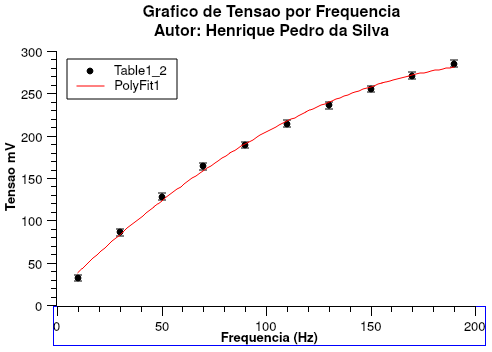
\includegraphics{Graph1.png}
\end{adjustbox}

\section{Tensão e corrente em elementos reativos}

\subsection{Fasores}

\subparagraph*{O que vamos ter eh que $\vec{V_m} = \vec{V_L} + \vec{V_R}$}
\subparagraph*{E também que a corrente estará defasada em $\pi/2$ em relação a tensão no indutor.}

\begin{adjustbox}{scale=0.9}
  \begin{tikzpicture}
    \begin{axis}[
      clip = false,
      xmin=0, xmax=2,
      ymin=0, ymax=2,
      axis lines=center,
      xlabel = $$, ylabel=$$,
      title={ },
      xtick={},
      xticklabels={}
      ytick={},
      yticklabels={}
      % xticklabel style = {anchor=south west},
      % xmajorgrids=true,
      % ymajorgrids=true,
      % grid style=dashed,
      ]


      % \addplot[domain=0:2*pi,color=blue, samples=100]{sin(deg(x))}
      % node[anchor=west, pos =0.7] {$3120$};



      \drawvector{0}{0}{1}{1}{Z}{true}{}{};
      \draw[line width=0pt,cyan,-stealth](axis cs: 0, 0)--(axis cs: 1, 1)  node[anchor= south east, pos =0.5] {$V_R e I_m$};

      \draw [cyan](axis cs: 0.3, 0) arc[start angle=0, end angle=45, radius=30]
      node[anchor= west, pos =0.6] {$wt$};


      \drawvector{0}{0}{-1}{1}{Z}{true}{}{};
      \draw[line width=0pt,cyan,-stealth](axis cs: 0, 0)--(axis cs: -1, 1)  node[anchor= south west, pos =0.5] {$V_L$};


      \drawvector{0}{0}{0}{1.41}{Z}{true}{}{};
      \draw[line width=0pt,cyan,-stealth](axis cs: 0, 0)--(axis cs: 0, 1.41)  node[anchor= south east, pos =0.5] {$V_m$};




    \end{axis}
  \end{tikzpicture}
\end{adjustbox}

\subsection{Medicoes $V_{ac}$ e $V_{bc}$}

\subparagraph*{Para altas frequências toda tensão do sistema estará no indutor, logo medir as tensões sobre o sistema me darão a tensão no indutor. E medir a tensão no resistor resultará em equivalência a medir a corrente no indutor.}

\subsection*{Reatancia}

\begin{equation}
  X_L = wL = 2 \pi f L = 2 \pi 300 = 1884 \varOmega
\end{equation}

\subparagraph*{Em regimes de alta frequência toda tensão do circuito estará no indutor, por isso esta diferença. Se a frequência fosse baixa o resultado seria o oposto.}
\subparagraph*{}

\subparagraph*{Verificando regra do divisor de tensão no regime CA.}

\begin{equation}
  \begin{aligned}
     & V_l             & \approx 4.99 V         \\
     & V_R             & \approx 71.64mV        \\
     & \frac{V_L}{V_R} & \approx 69.64          \\
     & X_L             & \approx 1884 \varOmega \\
     & V_R             & \approx 27 \varOmega   \\
     & \frac{X_L}{X_R} & \approx 69.7           \\
  \end{aligned}
\end{equation}

\subparagraph*{Logo podemos confirmar que os valores são coerentes.}

\subsubsection{Gráfico para tensão no indutor e corrente no indutor}
\subparagraph*{Aumentarei a magnitude da função que rege a corrente no indutor(a função vermelha) em 35 vezes, para deixar ela e a tensão na mesma escala. }

\subparagraph*{}

\begin{adjustbox}{scale=0.5}

  \begin{tikzpicture}
    \begin{axis}[
        ylabel={Tensao $V$},
        xlabel={Tempo $ps$},
        xmin = 0, xmax = 10,
        ymin = -6, ymax = 6.0,
        xtick distance = 2,
        ytick distance = 2,
        grid = both,
        minor tick num = 1,
        major grid style = {lightgray},
        minor grid style = {lightgray!25},
        width = 1\textwidth,
        height = 1\textwidth]
      \addplot[
        domain = 0:10,
        samples = 400,
        smooth,
        thick,
        blue,
      ] { 5 * sin(deg(2*pi*0.33* x))};
      \addplot[
        domain = 0:10,
        samples = 400,
        smooth,
        thick,
        red,
      ] {5* cos(deg(2*pi*0.33* x))};
    \end{axis}
  \end{tikzpicture}
\end{adjustbox}

\subparagraph*{Podemos então confirmar que a corrente esta de fato atrasada em $\frac{pi}{2}$}


\end{document}